\chapter{ext2}

\section{El sistema de archivos ext2}

Como dijimos anteriormente, ext2 es un filesystem basado en inodos. Los sistemas basados en inodos (explicaremos qué son los inodos más adelante) fueron creados para el sistema operativo UNIX, y son usados por todos sus descendientes.

El sistema ext2 (por \emph{second extended}) es un sistema de archivos diseñado e implementado para ser usado por el kernel de Linux. Fue inicialmente diseñado por Rémy Card como un reemplazo para el \emph{extended filesystem} (ext).

La implementación canónica de ext2 es el driver \emph{ext2fs} del kernel de Linux. Otras implementaciones existen en GNU Hurd, MINIX 3, y kernels de BSD.

ext2 fue el sistema de archivos por defecto en varias distribuciones de Linux, hasta que fue suplantado más tarde por ext3, que es un sistema de archivos con \emph{journaling}.
ext2 es aún hoy el sistema de archivos de elección para dispositivos de almacenamiento flash, dado que su falta de \emph{journal} mejora la performance y minimiza la cantidad de escrituras. 


Como ext2 fue diseñado e implementado para Linux, carece de una especificación canónica, por lo que esto dificulta la implementación de cero.

\subsection{Descripcion detallada de ext2}

Ahora analizaremos en detalle al sistema de archivos ext2. Como noit y Goldsmith en su trabajo práctico final también lo explicaron, amablemente me cedieron algunos gráficos y explicaciones que utilizaré a continuación (sobre todo de la parte de lectura), mientras que el resto de los gráficos y explicaciones fueron hechos por mí.

El sistema de archivos ext2 usa:
\begin{enumerate}
  \item bloques unidad básica de almacenamiento,
  \item inodos como medio de tener registro de archivos y objetos de ext2,
  \item  grupos de bloques para dividir lógicamente el disco en secciones más manejables,
  \item directorios para proporcionar una organización jerárquica de archivos,
  \item bitmaps de bloques e inodos para tener registro de bloques e inodos reservados,
  \item superbloques para definir los parámetros del sistema de archivo y su estado general.
\end{enumerate}

\subsubsection{Bloques}
Una partición o disco formateada con el sistema de archivos ext2 está dividida en pequeños grupos de sectores llamados \emph{bloques}. Estos bloques están agrupados, además, en unidades más grandes llamadas grupos de bloques.

El tamaño del bloque se determina cuando se formatea el disco y tiene impacto en la performance, el máximo tamaño de archivo posible y el máximo tamaño del sistema de archivos. Los tamaños de bloques más comunes son 1KiB, 2KiB, 4KiB and 8KiB, aunque los últimos 2 son los más usados en el último tiempo, dado el gran tamaño de los discos actuales.

\subsubsection{Grupos de bloques}

Los bloques se agrupan en grupos de bloques para reducir la fragmentación y minimizar la cantidad de movimientos del cabezal del disco cuando se lee una gran cantidad de datos consecutivos. La información sobre cada grupo se almacena en una tabla de descriptores que se encuentra en los bloques inmediatamente después del superbloque. 
Dos bloques cerca del inicio de cada grupo están reservados para \'el bitmap de uso de bloques y el bitmal de uso de inodos, que muestran cuales bloques e inodos estan siendo usados.
Como cada bitmap está limitado a un único bloque, esto significa que el tamaño máximo de un bloque de grupos es 8 veces el tamaño del un bloque.

Los bloques que siguen a los bitmaps en cada grupo de bloques están designados a la tabla de inodos para ese grupo y el resto son bloques de datos.


\begin{figure}
  \centering
  
\includegraphics[width=\textwidth]{img/block_structure.pdf}
  \caption{Estructura de un grupo de bloques.}
\end{figure}

\subsubsection{Inodos}

Como se ha dicho anteriormente, cada inodo representa un archivo o directorio. Los inodos contienen metadatos relevantes del archivo, a destacar:

\begin{itemize}
\item Los permisos de acceso. Incluyendo el clásico número octal de 3 cifras más otros 3 bits: Sticky bit que vale más que nada para forzar privilegios en los archivos de un directorio y los set process User/Group ID que setea los privilegios de Usuario/Grupo del archivo respectivamente al proceso si se ejecutase el archivo.
\item El tipo de archivo. Puede ser: Archivo común, directorio, block device, character device, socket, fifo o symlink.
\item El tamaño en bytes del archivo, vale para todos los tipos incluyendo directorios, más adelante se hablará de esto.
\item Los tiempos de acceso, borrado, creación, etc.
\end{itemize}

Por último lo más importante: contiene los números de los bloques que una vez concatenados formarían el archivo completo. Un lector atento se dará cuenta de que debido al tamaño fijo de los inodos, no sería posible representar archivos de gran tamaño ya que esto supondría almacenar muchos números de bloque, podemos despejar dicha inquietud con la siguiente imagen:

\begin{figure}
 \centering
 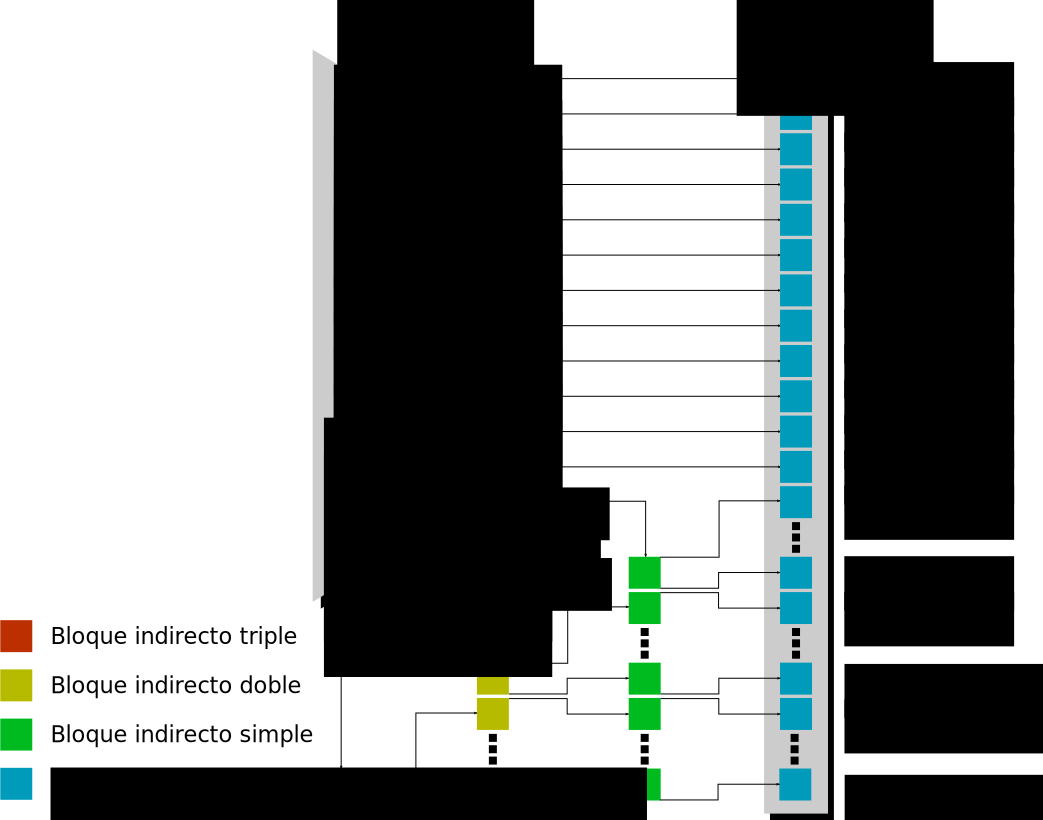
\includegraphics[width=\textwidth]{img/inodo.pdf}
 \caption{Estructura de un archivo junto con el inodo que lo representa, donde N es la cantidad de números de bloque que entran en un bloque. Esto es $N = \frac{block size}4$, ya que un número de bloque son 4 bytes.}
\end{figure}

\pagebreak

Hay dos tipos distintos de bloques, estos son:

\begin{description}
\item[De datos] Estos bloques forman el contenido del archivo. Se los identifica por su número absoluto en el filesystem como dijimos antes, en el inodo hay exactamente 12 de estos números (en orden) que apuntan a 12 bloques de datos, se los llama punteros a bloque directos. Si el archivo es lo suficientemente chico podrían no usarse los 12 punteros, en cuyo caso el resto de los números son inválidos. Los números que se les otorgaron en la imagen son relativos al archivo partiendo desde el 0, para poder comprender las distancias entre cada uno de los bloques mostrados y la magnitud que puede llegar a tener un archivo, no confundir con el número absoluto que los representa en el filesystem. Este número otorgado va a ser importante para entender la implementación más adelante.
\item[Indirecto] Estos bloques contienen punteros a otros bloques, esto es un arreglo de números de bloque que apuntan a otros bloques.
  Como dice la imagen, la cantidad de números de bloque que contienen es $\frac{block size}{4}$, ya que un número de bloque son 4 bytes. Podrían contener menos si el archivo no es lo suficientemente grande, en cuyo caso el resto de los valores son inválidos.
\end{description}

Y a su vez hay 3 tipos de bloques indirectos, en tres niveles de profundidad:

\begin{description}
\item[Simple] Contiene punteros a bloque directos. El inodo contiene un número de bloque apuntando a uno de estos (bn\_single en la imagen), si es que el tamaño del archivo es suficiente, el cual se lo denomina puntero a bloque simple.
\item[Doble] Contiene punteros a bloques simples, el inodo contiene un número de bloque apuntando a uno de estos (bn\_double en la imagen) si es que el tamaño del archivo es suficiente, el cual se lo denomina puntero a bloque doble.
\item[Triple] Contiene punteros a bloques dobles. El inodo contiene un número de bloque apuntando a uno de estos (bn\_triple) en la imagen, si es que el tamaño del archivo es suficiente, el cual se lo denomina puntero a bloque triple. Como es el nivel más grande posible de bloque indirecto solo puede haber uno por archivo, que es el apuntado por el inodo.
\end{description}

Gracias a esto, un inodo puede apuntar a una inmensa cantidad de bloques utilizando dichos bloques indirectos. La cantidad máxima de bloques que puede tener un archivo está delimitada por el tamaño de bloque, debido que a su vez esto delimita la cantidad de números de bloque dada por $N = \frac{block size}{4}$. En total nos quedan $12 + N + N^2 + N^3$ bloques de datos\footnote{Si tomamos los 12 bloques apuntados por el inodo, más los N bloques apuntados por el bloque indirecto simple, más los $N^2$ bloques apuntados por los $N$ bloques simples apuntados por el bloque indirecto doble, más los $N^3$ bloques apuntados por los $N^2$ bloques simples apuntados por los $N$ bloques dobles apuntados por el bloque indirecto triple}. Para bloques de 1KiB, esto es 16GiB de tamaño máximo de archivo, sin contar el costo de los bloques indirectos. \par

\subsubsection{Directorios}

Lo único importante que nos falta para entender cómo leer archivos de EXT2 son los directorios. En EXT2, estos son simplemente un tipo especial de archivo. Esto es, están representados por un inodo al igual que un archivo. Se los diferencia con el campo de tipo en el inodo como vimos anteriormente, y poseen una estructura particular dentro del contenido del archivo que define el contenido del directorio. \par
Notar que es aquí donde se almacenan los nombres de los archivos dentro del directorio y no en el inodo del archivo. Basta con conocer el inodo del directorio raíz, para poder comenzar a recorrer el filesystem. Alegrará saber que dicho inodo está reservado y es siempre el número 2. \par
Solo falta entender la estructura interna del directorio. Está formado por entradas de directorio una seguida de la otra, de tamaño variable. A su vez cada entrada tiene los siguientes campos:

\begin{description}
    \item[Inodo] El número de inodo del archivo al que estamos apuntando en esta entrada. Si es 0, la entrada se considera nula, esto es libre para ser usada en caso de tener que escribir una entrada o libre de ser ignorada en caso de tener que avanzar.
    \item[Tamaño de la entrada] El tamaño total de la entrada, contando todos los campos incluyendo el nombre y el padding necesario hasta la próxima entrada. Debe ser múltiplo de 4. Necesario para saber dónde está ubicada la siguiente entrada. Para decirlo de otro modo, la suma de estos campos de todas las entradas debería dar el tamaño del bloque.
    \item[Tipo de archivo] Esto originalmente era la parte alta del tamaño del nombre que es el siguiente campo, pero si se activa un flag en el superbloque (Que en general es activado de facto) se toma como tipo de la entrada. Notar que no son los mismos valores que en POSIX, sino un número del 0 al 7, ver tabla más adelante.
    \item[Tamaño del nombre] El tamaño del nombre que comienza justo después de este campo. Debido a que el otro campo es generalmente usado para el tipo nos da un tamaño de nombre máximo por archivo de 255 caracteres.
    \item[Nombre] El nombre del archivo, \textbf{no necesariamente un null terminated string}, hay que utilizar el tamaño del nombre para poder leerlo con seguridad.
    \item[Padding] Luego del nombre viene el suficiente padding para completar el tamaño de la entrada.
\end{description}

Los valores para los tipos son: \par

\begin{tabular}{r|l}
Valor & Tipo \\ \hline
0 & Indefinido/NULL \\ 
1 & Archivo común \\
2 & Directorio \\
3 & Char Device \\
5 & Block Device \\
4 & FIFO \\
6 & Socket \\
7 & Symbolic Link \\
\end{tabular} \\

Podemos ver un ejemplo de esto en la siguiente imagen:

\begin{figure}
  \centering
  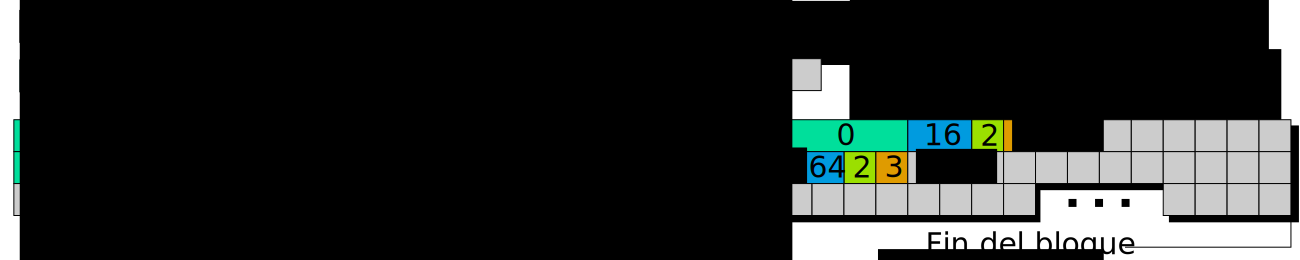
\includegraphics[width=\textwidth]{img/directorio.pdf}
  \caption{Estructura de un directorio raíz con bloques de 1KiB}
\end{figure}

Es un directorio raíz (Inodo 2), que sucesivamente, contiene las siguientes entradas:

\begin{description}
\item[.] Esta es una entrada estándar de tipo directorio (2) que poseen todos los directorios, la cual apunta al mismo directorio en cuestión, en este caso el inodo 2 que es este mismo.
\item[..] Esta es otra entrada estándar de tipo directorio (2) que poseen todos los directorios, apunta al directorio que contiene a este. Al ser el directorio raíz, este se apunta a sí mismo también, el número 2.
\item[Entrada Nula] La podemos detectar por el campo de inodo en 0. Podemos ignorarla en caso de lectura o usar el espacio vacío si quisiéramos escribir una entrada adicional en el directorio, siempre y cuando alcance el espacio.
\item[DeliriOS.bin] Este es un archivo, lo podemos detectar por el tipo (1). Está apuntando al inodo 23, si quisiéramos leerlo solo tenemos que cargar el inodo 23 y parsearlo correctamente. 
\item[var] Otro directorio (Tipo 2), ubicado en el inodo 30, si quisieramos leer su contenido tenemos que repetir el proceso actual pero con el inodo 30. Al ser la última entrada, necesariamente el tamaño abarca hasta el final del bloque. Para asegurarnos que llegamos al final, ya que podría haber más entradas en el bloque siguiente, chequeamos el tamaño del directorio (en este caso el raíz), si es 1024 entonces llegamos al final\footnote{Esto obliga a que el tamaño de los directorios sea siempre múltiplo del tamaño del bloque.}.
\end{description}


Con todo esto, ya podemos entender casi en completitud todo ext2, así que podemos pasar a ver las implementaciones del sistema de archivos.


Como dijimos anteriormente, ext2 carece de una especificación clara y canónica.
Todas las implementaciones de ext2 parten de analizar el código de la implementación de Linux e imitarlo.

Sin embargo, existe una documentación no oficial, escrita por Dave Poirier, que es en la que nos basamos para realizar este trabajo \cite{ext2doc}.

\subsection{Otras implementaciones}
\begin{puntos}
  \item Breve descripción de como otros sistemas operativos resolvieron el problema de los filesystems en general y ext2 en particular.
\end{puntos}



\newpage
\section{Nuestra implementación}

Este trabajo se trata sobre la implementación de la parte de escritura de ext2, es decir, las funciones que se ocupan de modificar el sistema de archivos de cualquier manera (creando, modificando y borrando archivos, en general). 

La parte de lectura del sistema de archivos (carga, interpretación de flags de opciones y lectura de archivos) puede encontrarse muy bien explicada en el trabajo de noit y Goldsmith.

\subsection{API de IO de DeliriOS}

Primero comencemos viendo la API de IO de DeliriOS, dado que esto nos va a permitir motivar y explicar todas las funciones de ext2 que implementamos.

\begin{lstlisting}[style=customc]
int64_t read(int64_t fd, void *buf, uint64_t count)
\end{lstlisting}
\begin{lstlisting}[style=customc]
int64_t write(int64_t fd, const void *buf, uint64_t count)
\end{lstlisting}
\begin{lstlisting}[style=customc]
int64_t seek(int64_t fd, int64_t offset, int64_t origin)
\end{lstlisting}
\begin{lstlisting}[style=customc]
int64_t tell(int64_t fd)
\end{lstlisting}
\begin{lstlisting}[style=customc]
uint8_t type(const char *path)
\end{lstlisting}
\begin{lstlisting}[style=customc]
int64_t create(const char *path, uint8_t filetype)
\end{lstlisting}
\begin{lstlisting}[style=customc]
int64_t remove(const char *path)
\end{lstlisting}
\begin{lstlisting}[style=customc]
int64_t truncate(int64_t fd, uint64_t length)
\end{lstlisting}
\begin{lstlisting}[style=customc]
int64_t open(const char *path)
\end{lstlisting}
\begin{lstlisting}[style=customc]
int64_t close(int64_t fd)
\end{lstlisting}
\begin{lstlisting}[style=customc]
int64_t opendir(const char *path)
\end{lstlisting}
\begin{lstlisting}[style=customc]
int64_t closedir(int64_t dd)
\end{lstlisting}
\begin{lstlisting}[style=customc]
int64_t rewinddir(int64_t dd)
\end{lstlisting}
\begin{lstlisting}[style=customc]
dir_entry * readdir(int64_t dd)
\end{lstlisting}


Como puede verse, es básicamente la API estándar de UNIX, nos inspiramos en ella porque de esta manera sería más fácil hacer programas en DeliriOS. 

Las funciones en las que nos concentraremos en este trabajo son: write, create, remove y truncate, dado que son aquellas para las cuales se necesita modificar el sistema de archivos.

El resto de las funciones son de lectura y fueron debidamente explicadas en el trabajo de noit y Goldsmith.


\subsection{Visión general de la implementación}

Pasaremos a dar una visión general del sistema de escritura, dado que el de lectura fue analizado en el trabajo de noit y Goldsmith.

Lo que necesitamos para una implementación exitosa de ext2 es, básicamente,

\begin{itemize}
  \item una cache de bloques,
  \item funciones que reserven bloques e inodos,
  \item funciones que escriban datos en bloques,
  \item funciones que modifiquen inodos.
\end{itemize}

La función central, que será la de escribir, tiene la siguiente pinta.


\begin{lstlisting}[style=customcmucho]
uint64_t fs_write(fs_info* info, fs_file* file,
                  const void *buffer, uint64_t count) {

    block_cache_set_dirty(info->head_cache, info->sb);
    block_cache_set_dirty(info->head_cache, info->gt);

    block_cache* cache = info->cache;
    uint64_t block_shift = info->block_shift;

    uint64_t block_size = 1 << block_shift;
    // remaining_after_eof es el numero de bytes que hay despues de que el
    // archivo  termina, porque no esta usando todo el bloque.
    // Cuando file->block_offset == block_size-1,
    // quiero que remaining_after_eof valga 0
    uint64_t remaining_after_eof =
        ( - file->remaining - file->block_offset) % block_size;
    // Escribo primero hasta el final del ultimo bloque, porque seguro
    // puedo hacerlo. fst_count es eso, la cantidad de bytes que puedo
    // escribir hasta quedarme sin bloques.
    uint64_t fst_count = MIN(count, file->remaining + remaining_after_eof);
    uint64_t written = 0;
    
    uint64_t size = count;
    while(size){
        // block_size - file->block_offset es lo que me queda por escribir
        // de un bloque.
        uint64_t to_copy = MIN(size, block_size - file->block_offset);
        // si me pase de lo que tenia alocado, tengo que pedir mas
        if(written >= fst_count){
            // pido un bloque, si devuelve distinto de 0, salgo
            if(ext2_request_block(info, file)) break;
        }
        void* block_ptr = block_cache_load_dirty(cache, file->block_number);
        void* base = (void*) ((uintptr_t) block_ptr + file->block_offset);
        memcpy(base, buffer, to_copy);
        block_cache_unload(cache, block_ptr);
        // me fijo cuanto tengo que correr el eof (file->remaining)
        if(file->remaining < to_copy){
            uint32_t eof_advanced = to_copy - file->remaining;
            block_cache_set_dirty(cache, file->inode);
            // actualizo el tamano del inodo, me fijo primero si hay overflow
            if(file->inode->size_low + eof_advanced < file->inode->size_low)
                file->inode->size_high++;
            file->inode->size_low += eof_advanced;
            file->remaining += eof_advanced;
        }
        ext2_seek(cache, block_shift, file, to_copy);
        buffer = (void*) ((uintptr_t) buffer + to_copy);
        size -= to_copy;
        written += to_copy;
    }
    return written;
}
\end{lstlisting}

Veamos como interviene cada punto que nombramos antes en esta función.

\begin{itemize}
  \item una cache de bloques: cuando queremos escribir un bloque, lo cargamos en la caché, lo escribimos, lo marcamos como "sucio" y lo descargamos, todas estas son funciones que deberán ser implementadas por la cache de bloques,
  \item funciones que reserven bloques e inodos: si el archivo no tiene más espacio disponible, debemos llamar a la función ext2\_request\_block, que se ocupa de reservar un bloque nuevo y actualizar todas las estructuras correspondientes,
  \item funciones que escriban datos en bloques: la función fs\_write en si,
  \item funciones que modifiquen inodos: la función fs\_write en si modifica inplace al inodo (actualizando por ejemplo el tamaño), pero también otras son necesarios otros procedimientos que serán utilizadas por funciones que creen y borren archivos.
\end{itemize}


Cuando se cargue un archivo para escritura, se reservaran PREALLOC\_BLOCK\_COUNT cantidad de bloques contiguos, de tal manera de tener un buffer de escritura que permita minimizar la fragmentación del archivo.

\subsection{Visión detallada de la implementación}

Pasaremos a describir función por función qu\'e hace cada una y que rol cumple en el sistema general.

\begin{lstlisting}[style=customc]
uint64_t fs_write(fs_info* info, fs_file* file, void *buffer, uint64_t count)
\end{lstlisting}

write escribe a partir del offset en el que se encuentra, la cantidad de bytes indicada por count del buffer.

Pueden pasar 3 cosas:
1. Entra la información y no hay que hacer ningún tipo de modificación al inodo.
2. Entra la información en los bloques que tenemos actualmente, pero el EOF se ve modificado, esto debe verse reflejado en el tamaño del archivo, que se guarda en el inodo.
3. La información no entra en los bloques asociados al archivo y debemos pedir más.

Es importante recordar que cierta información puede verse modificada (en particular el superbloque o la tabla de descriptores de grupos) si cambia la cantidad de bloques libres, entonces debemos marcar nuestras copias en la cache como /dirty/ para que sus cambios sean commiteados más tarde.

Cuando write encuentra que debe seguir escribiendo pero no tiene más bloques para hacerlo, llama a ext2\_request\_block, que se ocupa de poner un bloque para que write pueda seguir escribiendo sin hacer ningun tipo de trabajo extra.

\begin{lstlisting}[style=customc]
uint32_t ext2_request_block(fs_info* info, fs_file* file)
\end{lstlisting}

Se ocupa de calcular cuantos bloques son necesarios para brindar un bloque de datos (dado que por la estructura de ext2 pueden llegar a ser necesarios más de uno) para ello llama a ext2\_needed\_blocks.

Luego chequea si el archivo tiene suficientes bloques preasignados y en caso contrario llama a ext2\_balloc para que le asigne bloques al archivo.

Luego actualiza el inodo y asigna los bloques, armando correctamente la estructura de arbol del inodo de ext2, de tal manera de dejarle el bloque colocado de manera correcta a write para que pueda seguir escribiendo; para esto se utiliza la función ext2\_assign\_blocks.


\begin{lstlisting}[style=customc]
uint64_t ext2_needed_blocks(fs_info* info, fs_file* file)
\end{lstlisting}

Cuenta cuantos bloques reales necesito para devolver un bloque real de datos.


\begin{lstlisting}[style=customc]
uint32_t ext2_balloc(fs_info* info, fs_file* file)
\end{lstlisting}

Intenta alocar una constante fija de bloques para el archivo dado. La constante esta dada por PREALLOC\_BLOCK\_COUNT. Se podria usar tambien la constante que viene dada en el superbloque, pero es opcional.

El algoritmo es simple  e intenta minimizar la fragmentacion externa: intenta alocar desde el ultimo bloque utilizado por el archivo en adelante. Si no encuentra en el grupo actual, sigue con los grupos siguientes.

En caso de que el ultimo bloque del archivo sea el 0 (o sea, no tiene bloques asignados hasta ahora, por ejemplo, si el archivo estaba vacio) entonces se empezará a buscar desde el primer grupo.

Para llevar esto a cabo, se debe cargar el block usage bitmap de cada grupo de bloques y usar la funcion bitmap\_search\_zeros que busca n (en este caso PREALLOC\_BLOCK\_COUNT) bits en 0 juntos y devuelve el offset en el que se encuentran.

En caso de tener exito, los reserva usando la funcion ext2\_set\_resvd\_blocks.


\begin{lstlisting}[style=customc]
uint32_t ext2_assign_blocks(fs_info* info, fs_file* file)
\end{lstlisting}

Arma la estructura de arbol del inodo como corresponda para expandir el tamaño efectivo del archivo en 1 bloque. Para esto, tiene que eventualmente escribir nuevos bloques indirectos simples, dobles o triples.

Esta es definitivamente la función más compleja del driver de ext2 (junto con ext2\_unassign\_blocks que es prácticamente igual), sin embargo la idea es muy simple.

Se divide en todos los casos posibles y se asignan todos los bloques según corresponda.

\begin{lstlisting}[style=customc]
uint32_t ext2_set_resvd_blocks(fs_info* info, uint32_t from, uint32_t count, bool reserve)
uint32_t ext2_set_resvd_inodes(fs_info* info, uint32_t from, uint32_t count, bool reserve)
\end{lstlisting}

Estas funciones, muy similares, se ocupan de reservar/liberar bloques/inodos en el filesystem. Para eso, debe cargar el usage bitmap que corresponda y setear o limpiar los bits que correspondan, si se quiere reservar o liberar, respectivamente. 

El cuarto parametro indica si lo que se quiere hacer es reservar o desreservar. Si es true se reserva y si es false se libera.

\begin{lstlisting}[style=customc] 
uint32_t ext2_get_next_prealloc(fs_file* file)
\end{lstlisting}

Devuelve el proximo bloque de los prealocados por el archivo. Además actualiza la estructiura interna del archivo (dado que aumenta el puntero al primer bloque prealocado y disminuye la cantidad de bloques prealocados).


\begin{lstlisting}[style=customc]
uint32_t ext2_ialloc(fs_info* info, fs_dir* parent)
\end{lstlisting}

Busca, empezando por el grupo 0, algun inodo libre y devuelve su numero. 

\begin{lstlisting}[style=customc]
int64_t fs_create(fs_info* info, fs_dir* dir, dir_entry* file_info)
\end{lstlisting}

Crea un archivo en la carpeta pasada como parametro.

Para eso, pide un inodo con ext2\_ialloc y escribe la direntry correspondiente en los bloques de datos del inodo del directorio. Hay dos casos: se puede meter en el medio de la carpeta (porque hay entradas obsoletas en el medio) o debe ponerse al final.

Además, debe setear información como mode (permisos), creation time, modification time, entre otros.

\begin{lstlisting}[style=customc]
uint32_t ext2_unassign_block(fs_info* info, fs_file* file)
\end{lstlisting}

Le desasigna el bloque actual al archivo, que debe ser el ultimo (a menos que se quiera romper todo, o se sepa lo que se hace, dado que se rompe el invariante del archivo y queda un "hueco" en el medio). 

La lógica es la misma que la de ext2\_assign\_blocks, solo que se deben descargar aquellos indirectos que están cargados y no se necesitan más tambien.

\begin{lstlisting}[style=customc]
int64_t fs_truncate(fs_info* info, fs_file* file, uint64_t length)
\end{lstlisting}

Trunca al archivo y lo deja de tamaño length (bytes). Se asume que length es menor al tamaño del archivo (en caso de que no, se resuelve en la interfaz de io.c).

Para eso va hasta el final del archivo y va retrocediendo, desasignando bloques con ext2\_unassign\_block en caso de que sea necesario, actualizando toda la información que hace falta (el tamaño del archivo, que se encuentra en el inodo).

\begin{lstlisting}[style=customc]
int64_t fs_remove(fs_info* info, fs_dir* dir)
\end{lstlisting}

Borra el archivo apuntado actualmente por el directorio.

Hay que sobreescribir la entrada marcandola como invalida (seteando el numero de inodo en 0) y el deletion time acordemente. 


\begin{lstlisting}[style=customc]
uint32_t ext2_has_super(fs_info* info, uint64_t group)
\end{lstlisting}

Dice si un grupo del filesystem debe contener o no un backup del superbloque y el group descriptor table.

Si el filesystem tiene seteado la feature de sparse superblock, hay que chequear si el numero de grupo es 0 o potencia de 3, 5 o 7.


\begin{lstlisting}[style=customc]
uint32_t ext2_restore_backup(fs_info *info)
\end{lstlisting}

Escribe el superbloque y la group descriptor table en todos los grupos que deben tener el backup. Para eso, se va a usar ext2\_has\_super.


\begin{lstlisting}[style=customc]
uint64_t ext2_new_group(fs_info* info);
\end{lstlisting}
Esta funcion se encarga de inaugurar nuevos grupos de bloques. Debe tener en cuenta no pasarse del tamano del drive y mantener el superbloque esparso si asi corresponde.

De todos modos, esta funcion se usa en casos muy borde, cuando nos quedamos sin el espacio actual alocado en todo el filesystem. De hecho la especificacion ni siquiera es clara si esta operacion se puede hacer mientras el disco esta online y montado.

Esta función no fue implementada, simplemente está su signatura, dado que no es una función estándar (linux no asegura que esto no rompa la partición) y sólo algunos sistemas operativos la implementan.



\begin{lstlisting}[style=customc]
uint32_t ext2_group_first_block(fs_info* info);
\end{lstlisting}

Se trata de una función auxiliar que devuelve el primer bloque de un grupo. Es utilizada sobre todo para generar offsets

\begin{lstlisting}[style=customc]
int32_t ext2_add_direntry(fs_info* info, fs_dir* dir, char* filename, uint32_t inode, uint16_t filetype);
\end{lstlisting}

Esta función se utilizará para crear nuevos archivos dentro de un directorio.

Primero, esta función generará el struct con toda la información del archivo.

Simplemente esta función recorre todo el directorio (que recordemos que es un archivo) buscando alguna posición vacía. Cuando la encuentre, escribirá el struct generado anteriormente ahí. En caso de que no haya lugares vacíos, lo escribirá al final. Y en el caso de que no haya más lugar en el archivo, el archivo se extenderá con bloques nuevos.

\subsection{Cache de bloques}

La implementación general de la cache de bloques fue detallada en el trabajo de noit y Goldsmith. Sin embargo, debió ser cambiada para implementar la parte de escritura de ext2.

En particular, debieron ser agregadas las siguientes funciones.

\begin{lstlisting}[style=customcmucho]
static void block_cache_flush_entry(block_cache* cache, uint64_t entry_number) {
    block_cache_entry* vec = cache->vec;
    uint64_t block_number = vec[entry_number].number;
    hdd_write(block_number * cache->size_sectors + OFFSET_SECTORS, 
              cache->size_sectors, vec[entry_number].data);
    kfree(vec[entry_number].data);
    vec[entry_number].data = NULL;
    vec[entry_number].flags &= ~BLOCK_CACHE_DIRTY;
}
\end{lstlisting}

\begin{lstlisting}[style=customcmucho]
void block_cache_set_dirty(block_cache *cache, void *block_ptr) {
    if (block_ptr == NULL) 
        return;
    block_cache_entry* vec = cache->vec;
    // The index
    uint64_t i = 0;
    // We look it up and set the DIRTY flag on
    uint64_t count = cache->count;
    uintptr_t block_int = (uintptr_t) block_ptr;
    while (i < count) {
        // If it is any address inside the block
        if (block_int >= (uintptr_t) vec[i].data && 
            block_int < ((uintptr_t) vec[i].data + cache->size_bytes)){
            vec[i].flags|=BLOCK_CACHE_DIRTY;
            break;
        }
        i++;
    }

    if (i >= cache->count) {
        KERNEL_PANIC("Direccion %p no es valida en ningun bloque", block_ptr);
    }
}
\end{lstlisting}

Las funciones son bastante autoexplicativas.

La primera seatea el bloque en cuestión como no usado y lo escribe a disco. Además, libera el espacio en memoria que se pidió para guardar el bloque.

La segunda función marca un bloque como dirty. La única función de este procedimiento es permitir una optimización, dado que marcando bloques como dirty podemos ahorrarnos escrituras.
Si al liberar un bloque, este esta marcado como dirty, debemos escribirlo a disco. En cambio, si no está marcado como dirty, nos podemos ahorrar esta escritura, dado que sabemos que no fue modificado.


\subsection{Bitmap}

Para toda la manipulación de los bitmaps de uso de bloques e inodos debí implementar funciones de bitmaps. Estas se encuentran en utils/bitmap.c, y son muy fáciles de entender. Solamente pondré sus signaturas y una breve descripción de cada una.


\begin{lstlisting}[style=customc]
uint64_t clz8(int8_t byte)
uint64_t ctz8(uint8_t byte)
\end{lstlisting}

Cuentan cantidad de ceros delante/detras del número (count leading/trailing zeros). Esperan un numero de 8 bits.




\begin{lstlisting}[style=customc]
uint64_t bitmap_count_zeros(const void* const _bitmap, uint64_t size, uint64_t offset)
\end{lstlisting}

Cuenta la cantidad de ceros consecutivos en el bitmap desde offset hasta size.
Toma como parametros el bitmap en cuestion, el tamaño del bitmap en bits y desde que bit empezar a buscar ceros.



\begin{lstlisting}[style=customc]
uint64_t bitmap_search_zeros(const void* _bitmap, uint64_t size, uint64_t offset, uint64_t count)
\end{lstlisting}

Busca count cantidad de bits en cero en el bitmap. Recibe como parámetros el bitmap en cuestión, el tamano del bitmap en bits, desde que bit empezar a buscar ceros y cuántos ceros buscar.

Devuelve la posición a partir de la cual encontro los bits. Si es size, significa que no encontro.



\begin{lstlisting}[style=customc]
uint64_t bitmap_set_bits(const void* _bitmap, uint64_t size, uint64_t offset, uint64_t count)
uint64_t bitmap_clear_bits(const void* _bitmap, uint64_t size, uint64_t offset, uint64_t count)
\end{lstlisting}

Modifica el bitmap poniendo en 1 (o 0, si es clear) count cantidad de bits de offset en adelante.

Devuelve 0 si salió todo bien, 1 si se pasó de size y 2 si ya estaban seteados en 1 (o 0, si es clear).

\subsection{Testing}

Para testear, diseñamos un subsistema especial, que nos permitiera probar la correctitud de las funciones implementadas desde afuera de delirios. Para esto, utilizamos la clásica técnica de dependency injection.

Tenemos una imagen de ext2 en un archivo (hdd.img), y lo que hacemos es abrirla como si fuera un archivo común y corriente, y guardamos su file handler en una variable global llamada fp.

Luego, pasamos a lo vital de la dependency injection: overloadeamos as funciones hdd\_read y hdd\_write de la siguiente manera.


\begin{lstlisting}[style=customcmucho]
void hdd_read(uint32_t lba_address, uint32_t sectors, void* buffer) {
    fseek(fp, lba_address * ATA_SECTSIZE, SEEK_SET);
    fread(buffer, ATA_SECTSIZE, sectors, fp);
}
\end{lstlisting}

\begin{lstlisting}[style=customcmucho]
void hdd_write(uint32_t lba_address, uint32_t sectors, void* buffer) {
    fseek(fp, lba_address * ATA_SECTSIZE, SEEK_SET);
    fwrite(buffer, ATA_SECTSIZE, sectors, fp);
} 
\end{lstlisting}

De esta manera, cuando las funciones de ext2 y de la cache de bloques las llamen, van a pensar que estan leyendo de un disco, mientras que simplemente estamos escribiendo un archivo.

Así, podemos testear todas las funciones que implementamos con extrema facilidad. En particular, todas las funciones presentadas en este informe tienen tests de todo tipo: funcionales, de error, de carga, entre otros.


